\chapter{Set theory}

In the following, we will be going through some fundamental aspects of set theory, the mathematical study of sets. Modern set theory is a very abstract field, and to make matters more confusing, set theory is usually formulated using a formal language of logic. And in turn, formal languages of logic are specified, both syntactically and semantically, through the use of set theory. Thus, there is a chicken-or-the-egg scenario going on. To steer clear of these issues, we will be explaining set theory in plain English terms. 

\section{Sets and membership}

Set theory is all about sets. For now, we can say that sets are some specific collections of things. These things can be of any sort, including sets themselves. Going back to file systems, in some important aspects, sets are like folders, which may contain other folders, which in turn may contain other folders, and so on. In fact, sets are denoted just as we denoted folders in our language $\mathcal{L}_f$; using curly braces. Thus, the following is a set:
\[
\set{\text{Peter}, \text{Leo}, \text{Taylor}, \text{Curtis}}
\]

Sets have \textit{members}. The members of a set are those things that are in the set. So the members of the set $\set{\text{Peter}, \text{Leo}, \text{Taylor}, \text{Curtis}}$ are Peter, Leo, Taylor, and Curtis. Set membership is denoted by $\in$. So for example, 
\[
\text{Peter} \in \set{\text{Peter}, \text{Leo}, \text{Taylor}, \text{Curtis}}
\]
We can denote sets by using capital letters. The first choice is usually $S$ (you can guess why...). This makes it easier to talk about them. So for example:
\begin{gather*}
	S=\set{\text{Peter}, \text{Leo}, \text{Taylor}, \text{Curtis}}\\
	\text{Peter} \in S
\end{gather*}
Similarly, we can denote something not being in the set by using $\notin$. So for example:
\[
\text{Henry} \notin S
\]
So far, this is rather simple. Now let's look at some complications. 

Sets are \textit{extensional} entities. This is a fancy word to say that all a set depends on is what its members are. So in a set, there is no ordering between its members, and it doesn't matter whether the set is represented as having some members twice (or however many times). Each member is only counted once, in whatever order. So for example:
\begin{align*}
\set{\text{Peter}, \text{Leo}, \text{Taylor}, \text{Curtis}}&=\set{\text{Peter}, \text{Peter}, \text{Leo}, \text{Taylor}, \text{Curtis}}\\
\set{\text{Peter}, \text{Leo}, \text{Taylor}, \text{Curtis}}&= \set{\text{Curtis}, \text{Leo}, \text{Peter}, \text{Taylor}}
\end{align*}

\begin{defn}[Set extensionality] Two sets $S$, $Q$, are identical if they have exactly the same members. That is, for all $x$, $x \in S$ if, and only if, $x \in Q$. If $S$ and $Q$ are identical sets, we write $S=Q$.
\end{defn}

\begin{exc}
Determine whether the following sentences are true or false. In each case, explain your reasoning. 

\begin{enumerate}
	\item $a \in \{b, g, h, a\}$;
	\item if $\{b, g, h, a\}=S$, then $b \in S$;
	\item the set $\{b, b, b\}$ has exactly one member;
	\item if $Q=\set{3, 5, 7, 7}$, then the sum of its members is $22$;
	\item if $S=\set{a, h, q, r}$, then $\text{Peter} \notin S$.
\end{enumerate}
\end{exc}

There is one set that is unlike others, denoted $\emptyset$. This is the empty set. The empty set is so-called because it is, you guessed it, empty. In other words, it has no members. So for any candidate member $x$, $x \notin \emptyset$. 

Now sets can be members of other sets, and it is very important to be clear whether something is in a set, or it is in another set that is part of another set, and so on. Note: since $\emptyset$ is a set, it can also be a member of other sets. Let's look at an example: 
\begin{align*}
	S&=\set{a, b, c, \set{a, d}, d, \emptyset}\\
	Q&=\set{\set{a, b, c}, \set{d}, d, \emptyset}
\end{align*}

Now $S$ and $Q$ are not the same set. They do share \textit{some} elements, but they differ in others. Since they do not have the same elements, they are not the same set. In particular, $\emptyset \in S, Q$, and $d \in S, Q$. But note that $a, b, c \notin Q$. What \textit{is} in $Q$ is the \textit{set} \set{a, b, c}. Conversely, $a, b, c \in S$, but not $\set{a, b, c}$. Similarly, $\set{d} \in Q$ but $\set{d} \notin S$, though again, $d \in S, Q$. 

\begin{exc}
	Determine whether the following expressions are true or false. In each case, explain your reasoning. 
	
	\begin{enumerate}
	\item $S=\set{\emptyset}$ has no members;
	\item $\emptyset$ has exactly one member, $\emptyset$;
	\item $S=\set{a, b, \set{b}, \set{\set{a, b}},b, \set{\emptyset}}$ has exactly $5$ members;
	\item the sets $\emptyset$, $\{\emptyset\}$, and $\set{\emptyset, \emptyset}$ are pairwise distinct (that is, no two of them are the same set);
	\item if $S=\set{a, \set{a}, \set{a, \set{a}}}$ and $Q=\set{a, \set{a, \set{a}}}$, then every member of $Q$ is a member of $S$;
	\item if $S=\set{a, \set{a}, \set{a, \set{a}}}$ and $Q=\set{a, \set{a, \set{a}}}$, then every member of $S$ is a member of $Q$. 
	\end{enumerate}
\end{exc}

\section{Sets and subsets}

Now that we know what sets are, how they are represented, and which sets are the same, we can talk about another important relationship between them. That is, one set being the \textit{subset} of another set. If we have a set, say $S$, and a set, say $Q$, then $S$ is a subset of $Q$ if every member of $S$ is also a member of $Q$. So for example, if $S=\{a, b,c\}$ and $Q=\{a, b, c, d\}$, then $S$ is a subset of $Q$. 

\begin{defn}[Subset]
If $S$ and $Q$ are sets, and every member of $S$ is also a member of $Q$, then $S$ is a \textit{subset} of $Q$ ($Q$ is a \textit{superset} of $S$). In such cases, we write $S \subseteq Q$ (or $Q \supseteq S$). 
\end{defn}

One thing that is important to note with the subset relation is that it does not exclude the possibility that two sets are the same. Indeed, there is a general fact concerning this matter. Namely, if $S$ and $Q$ are sets, and $S \subseteq Q$ and $Q \subseteq S$, then $S=Q$. In other words, if $S$ is a subset of $Q$, and $Q$ is a subset of $S$, then $S$ and $Q$ are identical. 

\begin{exc}
Explain why it is the case that if $S$ and $Q$ are sets, and $S \subseteq Q$ and $Q \subseteq S$, then $S=Q$.
\end{exc}

Now if we wanted to specify explicitly that one set is a subset \textit{and} not equal to another set, we can use the symbol $\subset$, which stands for `proper subset'. Proper subsets are just like subsets, except they come with the additional caveat that the two sets are not the same. In other words, $S \subset Q$ is just a short way to say that $S \subseteq Q$ and $S \neq Q$ (it is not the case that $S = Q$). 

One thing that usually trips up people new to set theory (and sometimes, even those who aren't) is differentiating between $\in$ and $\subseteq$, that is, differentiating between one set being a member of another set, and one set being a subset of another set. It's important to make sure you can distinguish between the two!

\begin{exc}
Determine whether the following expressions are true or false. In each case, explain your reasoning. 

\begin{enumerate}
	\item if $S=\{1, 7, 3\}$ and $Q=\{1, 3\}$, then $Q \subseteq S$;
	\item if $S=\{1, 7, 3\}$ and $Q=\{7, 1, 3\}$, then $S \subseteq Q$ and $Q \subseteq S$;
	\item if $S=\{a, b\}$, and $Q=\set{\set{a, b}}$, then $S \in Q$;
	\item if $S=\{a, b\}$, and $Q=\set{\set{a, b}}$, then $S = Q$;
	\item if $S=\{a, b, \set{a, b, c}\}$, and $Q=\{a, b, c\}$, then $Q \subseteq S$;
	\item if $S=\{h, f, \set{g,\set{f}}\}$ and $Q=\set{g, \set{f}}$, then $Q \subseteq S$. 
	\item if $S=\{a, d, h\}$, then $S \subseteq S$;
	\item if $S=\{d, b, c\}$, then $S \subset S$.
\end{enumerate}
\end{exc}

Finally, we must mention the case of $\emptyset$. Though it may sound a bit strange at first, $\emptyset$ is a subset of \textit{every} set, including itself! Why? Because all its members are members of every other set. Why? Because it has none! Thus, in general, for every set $S$, $\emptyset \subseteq S$. On the other hand, it is \textit{not} the case that every set has $\emptyset$ as its member. Some sets may, some sets may not. So for example, if we take $S=\set{\set{\emptyset}}$, $\emptyset$ is not a member of $S$, but $\emptyset \subseteq S$. Moreover, $Q=\{\emptyset\}$ is a member of $S$, and $\emptyset \subseteq Q$ \textit{and} $\emptyset \in Q$. 

\section{Sets and properties}

Since our semantics will be formulated in set theory, sets will play a central role in it. One of these roles will be to represent \textit{properties}. Some properties are `is red', `is a mammal', `is 6 feet tall', `is the friend of Honghui', and so on. These properties are either `had' by certain things or not. The technical term is `exemplify'. So for example, every human has or exemplifies the property `being a mammal', since every human is a mammal, but not every human is exactly 6 feet tall, so some have or exemplify the property `is 6 feet tall', and some do not. 

The simplest way to formally represent these properties is just to have a set of all those things that exemplify that property. So for example, one may form the set $H$ of all (and only) those things that are human (exemplify `is a human'), and thus the set $H$ will represent the \textit{property} `is a human'. Similarly, one can represent the property `is a mammal' by a set $M$ consisting of all (and only) the things that are mammals. 

Now let's look at some examples. Taylor Swift will be in the set $H$ and the set $M$, since she is a human and a mammal (exemplifies the property `is a human' and `is a mammal'). However, if $S$ represents the property `is 6 feet tall', she will not be in $S$, since she is not 6 feet tall (apparently, she's 5'11''). The same goes for Jay-Z, since he is also a human and a mammal, and also not 6 feet tall (apparently, he is 6'2''). On the other hand, if we take Jay-Z's Corvette C-1, it is neither in $H$, nor $M$, nor $S$, since it is a car that does not have any of these properties. 

You can also look at which properties (understood as sets) are subsets of which other properties (understood as sets). For example, since every human is a mammal, the property `is a human' is a subset of the property `is a mammal', since every member of $H$ is a member of $M$. Indeed, $H$ is a proper subset of $M$, since there are many mammals that aren't human. In other words, there are many animals in $M$ not in $H$. 

\fpboxstar{
There is a famous philosophical problem when it comes to identifying properties with sets. Namely, there are some properties that we would say are distinct, though they apply to exactly the same things, and hence they would be identified with the same set. For example, the property `is the the first rapper to be inducted into the Songwriters Hall of Fame' and the property `is the first solo living rapper inducted in the Rock and Roll Hall of Fame' seem to be different properties, yet if we identify properties with sets, they are the \textit{same} set $\set{\text{Jay-Z}}$, so they are the same property. The wrong result! However, for our purposes (which is doing logic), it is okay to identify properties with sets. 
}

We will return to the topic of properties and semantics in the next chapter. 

\section{Ordered sets and Cartesian products}

Antoher thing that is especially important in the set theoretic foundations of logic is the notion of an ordered set. As mentioned above, sets are, by nature, unordered. Again, if $S=\{a, b\}$ and $Q=\{b, a\}$, then $S=Q$. But sometimes, we \textit{do} want to talk about ordered sets, where the ordering of the members does matter. Ordered sets to the rescue! 

Unlike normal sets, which are enclosed by curly braces, ordered sets are denoted with the angled braces $\langle$ and $\rangle$. For example, if we take the ordered set of $a$, $b$, and $c$ in just this order, we can write $\langle a, b, c \rangle$. The ordered set $\langle c, b, a \rangle$ is distinct from this, since it has its order reversed. 

The fact that they are ordered is not the only difference between normal sets and ordered sets. Another important difference is that for ordered sets, duplicates do count for something. Namely, the ordered set $\langle a \rangle$ and the ordered set $\langle a, a\rangle$ are not the same ordered set (and in general, not the same set either). So in general, unlike normal sets, ordered sets can be distinguished at face value. 

Sometimes, some ordered sets are called ordered $n$-tuples, where $n$ is the number of members of the ordered set. For small $n$, we have specific words for these tuples, but after a while, they become unwieldy, and aren't generally used. So for example, $\langle a, b \rangle$ is an ordered \textit{pair}, $\langle a, b, c \rangle$ is an ordered \textit{triple}, $\langle a, b, c, d \rangle$ is an ordered \textit{quadruple}, and so on. 

Another important notion in set theory is the Cartesian product of two sets. If $S$ and $Q$ are two sets, their Cartesian product is denoted by $S \times Q$. Indeed, Cartesian products are one way in which one may `make' ordered sets out of regular sets. In particular, if $S$ and $Q$ are sets, then $S \times Q$, their Cartesian product, is the set of all ordered pairs such that their first member is in $S$, and their second member is in $Q$. 

For example, suppose $S=\set{a, b}$ and $Q=\set{1, 2}$. Then, $S \times Q=\set{\oset{a, 1}, \oset{a, 2}, \oset{b, 1}, \oset{b, 2}}$. Again, it is just the \textit{set} of all ordered pairs with the first member of the pair in $S$, and the second in $Q$. 

Now importantly, $S$ and $Q$ need not be different, so that $S\times S$ is itself a set, the set of all ordered pairs made up of members of $S$. So for example, if $S=\{a, b, c\}$, then $S \times S=\set{\oset{a, b}, \oset{a, c}, \oset{b, a}, \oset{b, c}, \oset{c, a}, \oset{c, b}, \oset{a, a}, \oset{b,b}, \oset{c,c}}$. From this, you may see why taking the Cartesian product of two sets is denoted by the $\times$ (`product') operator, since if a set $S$ has $3$ members, then $S \times S$ will have $9$ members, and so on. We can also write this more succinctly as $S^2$, and $S^3$, etc. 

\fpboxstar{The name `Cartesian product' comes from an interesting historical fact. `Cartesian' refers to René Descartes, one of the most important philosophers in history, who was also a pioneering mathematician. As such, he devised the coordinate system you probably already know from mathematics. What does this have to do with Cartesian products? For example, think of the Cartesian product of $\mathbb{N} \times \mathbb{N}$. Its members are all pairs of natural number $\oset{n, k}$. Like $\oset{3, 4}$, $\oset{1,1}$, $\oset{6, 0}$. But of course, these are exactly the coordinates of a two-dimensional coordinate system on the natural numbers.}

\begin{exc}

Answer the following questions. For each question, don't forget to explain your reasoning. 	

	\begin{enumerate}
		\item What is the Cartesian product of the set $S=\{Lebron, Taylor\}$ with itself?
		\item Is the set $Q=\set{\oset{Taylor, Lebron}, \oset{Lebron, Leo}}$ a subset of $S \times S$?
	\end{enumerate} 
\end{exc}

\fpboxstar{
You may be wondering what the relationship is between sets and ordered sets. In set theory books, it is customary to show how ordered sets are definable from the notion of a set. In particular, one can define the ordered pair $\oset{a, b}$ to be the set $\set{\set{a}, \set{a, b}}$. This is a kind of encoding, which allows one to determine the order of the two elements $a$ and $b$ from the set of two sets that are themselves not ordered in any way. This kind of definition can be further generalized to cover any $n$-tuple (for any $n$), by iterating the ordered pairs. For example, an ordered triple would be the ordered pair of an ordered pair and a third thing. That is, $\oset{a, b, c}=\oset{\oset{a, b}, c}$. It is then possible to further analyze $\oset{\oset{a, b}, c}$ according to our set-based definition of ordered pairs. There are alternative ways to do essentially the same thing. 
}

\section{Ordered sets and relations}

The reason why ordered pairs, and ordered sets in general, are useful, is because they allow us to encode more structured information than just normal, unordered sets. For example, suppose we want to represent the fact that for three people, Jamal, Kerry, and Zoltan, some are friends with one another, and some aren't. For each person, we can create the set of friends of that particular person with normal sets. 

Suppose the following. Jamal is friends with Kerry, Zoltan is friends with Jamal, but Kerry is not friends with Zoltan. For each person, we may specify the set of friends they have, so that $S_J=\set{\text{Kerry}, \text{Zoltan}}$, $S_K=\set{\text{Jamal}}$ and $S_Z=\set{\text{Jamal}}$. These would be the properties `is the friend of Jamal', `is the friend of Kerry' and `is the friend of Zoltan', respectively. 

However, with ordered sets, we can do all of this in one set, representing the \textit{relation} `is friends with'. First, we can immediately specify: 
%
\[F=\set{\oset{\text{Jamal}, \text{Kerry}}, \oset{\text{Kerry}, \text{Jamal}}, \set{\text{Zoltan}, \text{Jamal}}, \oset{\text{Jamal}, \text{Zoltan}}}\]
%
Note that we included, for both Jamal and Kerry, and Jamal and Zoltan, the two names in both configurations. This is useful, since we may desire to add lopsided relations that are not mutual. For example, suppose we want to represent that Jamal is friends with Kerry, and Kerry is friends with Jamal, Zoltan is friends with Jamal and Jamal is friends with Zoltan, and also that Kerry thinks Zoltan is her friend, but Zoltan does not view Kerry as a friend. Then, we can encode this as: 
%
\[F'=\set{\oset{\text{Jamal}, \text{Kerry}}, \oset{\text{Kerry}, \text{Jamal}}, \set{\text{Zoltan}, \text{Jamal}}, \oset{\text{Jamal}, \text{Zoltan}}, \oset{\text{Kerry}, \text{Zoltan}}}\]
%
Here, $F'$ represents the `is friends with' relation again (in a different situation). But using this blueprint, any relation can be represented, starting from such pairs to more elaborate ones, like `$x$ is in between $y$ and $z$', which would be a set of triples, and so on. 

Related to sets of ordered pairs are three important notions that are usually specified. First, a relation may be \textit{reflexive}. This means that for any $x$ (that occurs in the `field' of a relation $R$, see below), $\oset{x, x} \in R$. For example, if $L$ encodes the `loves' relation, and everyone loves themselves, then for every person $x$, $\oset{x, x} \in L$. This way, $L$ would be reflexive. On the other hand, if there is a person $y$ such that $\oset{y, y} \notin L$, then $L$ would not be reflexive, because there would be a person who does not love themselves. 

\begin{figure}[h]\centering
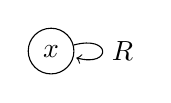
\begin{tikzpicture}
	\begin{scope}[every node/.style={circle,draw}]
	\node (a) {$x$};
\end{scope}

\path [->] (a) edge[loop right] node[right] {$R$} (a);
\end{tikzpicture}
\caption{A graphical representation of an instance of reflexivity}
\end{figure}

Second, a relation may be symmetric, if whenever $\oset{x, y} \in R$, $\oset{y, x} \in R$ as well. This was already illustrated above with our three friends, Jamal, Kerry, and Zoltan. Specifically, $F$ was a relation that was symmetric, since whenever $x$ was a friend of $y$, $y$ was a friend of $x$. On the other hand, $F'$ was not symmetric, since there was a person, Kerry, who was friends with Zoltan, but Zoltan was not friends with Kerry. 

\begin{figure}[h]\centering
\begin{tikzpicture}
	\begin{scope}[every node/.style={circle,draw}]
		\node (a) {$x$};
		\node [right=2cm of a] (b)  {$y$};
	\end{scope}
	
	\path [->] (a) edge[bend left=60] node[below] {$R$} (b);
	\path [->] (b) edge[bend right=270] node[above] {$R$} (a);
\end{tikzpicture}
\caption{A graphical representation of an instance of symmetricity}
\end{figure}

Finally, a relation may be transitive. Transitive relations are everywhere in logic, though they are not always apparent. A transitive relation is more elaborate than the above two, since it is specified between three things. Namely, a transitive relation is such that if $\oset{x, y} \in R$, and $\oset{y, z} \in R$, then $\oset{x, z} \in R$. One relation that is usually transitive is airplane travel with connections. Suppose you can travel by plane from New York to Los Angeles, and from Los Angeles to Tokyo. Then, that also means that you can travel from New York to Tokyo (with a connecting flight in Los Angeles). In other words if $A$ represents the set of all pairs of cities reachable by air travel, if $\oset{\text{NYC}, \text{LA}} \in A$, and $\oset{\text{LA}, \text{Tokyo}} \in A$, then $\oset{\text{NYC}, \text{LA}} \in A$. Since this holds for every three cities, the relation $A$ is transitive. Incidentally, this relation is also symmetric, since flights go back and forth (or perhaps in larger circles).  

\begin{figure}[h]\centering
\begin{tikzpicture}
	\begin{scope}[every node/.style={circle,draw}]
		\node (a) {$x$};
		\node [right=2cm of a] (b)  {$y$};
		\node [right=2cm of b] (c)  {$z$};
	\end{scope}
	
	\path [->] (a) edge[bend left=60] node[below] {$R$} (b);
	\path [->] (b) edge[bend left=60] node[below] {$R$} (c);
	\path [->] (a) edge[bend right=30] node[below] {$R$} (c);
\end{tikzpicture}
\caption{A graphical representation of an instance of transitivity}
\end{figure}

\fpboxstar{%
If you have taken an introductory logic course before, you may remember the connective `$\rightarrow$', standing for `if ..., then ...'. You may also remember that in your proof system, you could show that if you had as premises $X \rightarrow Y$ and $Y \rightarrow Z$, then you could derive $X \rightarrow Z$. Some systems even have a dedicated rule for this, called the `hypothetical syllogism' or `chain rule'. Now all this rule says is that $\rightarrow$ is transitive! In other words, if you take the set $I$ of all pairs $X$, $Y$ of propositions where $X \rightarrow Y$, and $\oset{X, Y}, \oset{Y, Z} \in I$, then $\oset{X, Z} \in I$ (at least in classical logic). 
}

Note that relations can have many `places', meaning they may be said to hold between several different things. A $2$-place relation, as noted above, is a set of pairs, since it holds (or does not hold) between two things. But you may take other relations like `$x$ is in between, $y$ and $z$', which would be a $3$-place relation, and its representation would be a set of triples $\oset{x, y, z}$, because it holds (or does not hold) between 3 things. So in general, an $n$-place relation will be identified with a set of $n$-tuples, since it holds (or does not hold) between $n$ different things. Notice that in each case, an $n$-place relation $R$ is a subset of some set $S$ taken $n$ times with itself, i.e., $R \subseteq S^n$. 

\begin{defn} \label{refsymtran}
Let $S$ be any set. An $n$-place \textit{relation} $R$ \textit{defined on} $S$ is a subset of the Cartesian product $S^n$, that is, the product of $S$ taken $n$ times with itself. In such cases, we call $S$ the \textit{field} of $R$. 

If $R$ is a two-place relation with field $S$, then: 
\begin{enumerate}
	\item if for all $x \in S$, $\oset{x, x} \in R$, then $R$ is \textit{reflexive};
	\item if for all $x, y \in S$, if $\oset{x, y} \in R$, then $\oset{y, x} \in R$, $R$ is \textit{symmetric};
	\item if for all $x, y, z \in S$, if $\oset{x, y}, \oset{y, z} \in R$, then $\oset{x, z} \in R$, $R$ is \textit{transitive}. 
\end{enumerate}

If the relation $R$ is reflexive, symmetric, and transitive, we say it is an \textit{equivalence relation}.
\end{defn}

\begin{exc}
Determine for each claim whether it is true or false. Don't forget to explain your reasoning, using the above definitions! Note: these are more philosophical questions regarding the exact meaning of some relations expressed in English. There may not be a single correct answer for each. 

\begin{enumerate}
	\item the relation `$x$ is related to $y$ by blood' is transitive;
	\item the relation `$x$ is an ancestor of $y$' is transitive;
	\item the relation `$x$ is right of $y$' is transitive on a 1-dimensional plane;
	\item the relation `$x$ is right of $y$' is transitive on a 2-dimensional plane;
	\item the relation `$x$ is a brother of $y$' is symmetric;
	\item the relation `$x$ is a sibling of $y$' is symmetric;
	\item the identity relation `$=$' is reflexive, symmetric, and transitive. 
\end{enumerate}
\end{exc}

\section{Functions as sets of ordered pairs}

Another thing that you will need to know as we move forward is a bit about \textit{functions}. Functions may seem like mysterious entities, but set theoretically speaking, they are really quite simple. After all, what a function does is it takes an \textit{input}, and provides a single \textit{output}. For example, if we take the function $+2$, and apply it to the number $3$, we get $5$. There are various ways of specifying the $+2$ function, like $f(n)=n+2$, or $f: n \mapsto n+2$, but the only thing that is important is that there are a bunch of inputs, and for each input, there is just one output. So if $f$ is the $+2$ function, then $f(3)=5$.
 
\fpboxstar{
Perhaps somewhat confusing to the untrained eye is the fact that $f(3)$, as specified above is, by itself, the same as the number $5$. So in this context, it makes sense to write things like $f(3)+3=8$, or $f(3) \in \mathbb{N}$. 
}  

Functions can be represented in set theory by sets of ordered pairs. These ordered pairs essentially represent a list of all input-output pairs that a function is made up of. For example, if we take the $+2$ function again, defined on the natural numbers $\mathbb{N}$, set theoretically, it would be the set of all the following ordered pairs:
\begin{gather*}
	\oset{0, 2}\\
	\oset{1, 3}\\
	\oset{2, 4}\\
	\oset{3, 5}\\
	\oset{4, 6}\\
	\vdots
\end{gather*}
%
Or in one line, $\set{\oset{0, 2}, \oset{1, 3}, \oset{2, 4},	\oset{3, 5}, \oset{4, 6}, ...}$. Again, this is just a list of all possible input-output pairs for the function. 

\fpboxstar{Note the use of `$...$' in specifying the $+2$ function. Since the function $+2$ is defined on all natural numbers, naturally, its set-theoretic representation will be an infinitely large set! What the dots represent is that the list goes on forever, since for any natural number, you can always just add $2$ and get another one.}

One thing that you need to keep in mind is that not any set of ordered pairs constitutes a function. In particular, functions are those sets of ordered pairs where for each input, there is only one output. One way to formulate this idea is to say that if there is an input to the function, and seemingly two different outputs, then those two seemingly different outputs must be the same. Hence:

\begin{defn}[Function] A \emph{function} $f$ is a set $S$ of ordered pairs such that if $\oset{a,b} \in S$ and $\oset{a, c} \in S$, then $b=c$. The set $A$ of all $a$ such that $\oset{a, b} \in S$ is called the function's \emph{domain}, while the set $B$ of all such $b$ is called its \emph{range} or \emph{image}. A function's codomain $C$ (if specified) is a superset of its range. 
	
We may write $f: A \to C$ to specify $f$ to be a function with domain $A$ and codomain $C$. If $\oset{a, b} \in S$, we may write, alternatively, that $f(a)=b$, or that $f: a \mapsto b$.   
\end{defn}

\begin{exc}
Is every function a relation? Is every relation a function? In your answer, explain your reasoning. 
\end{exc}


The above definition ensures that whatever conforms to that specification is an actual function. On the other hand, one can introduce more restrictions on these sets, to define certain special classes of functions. 

Let's start with some useful terminology. According to the above definition, there are no functions which are one-to-many, in the sense of assigning many outputs to one input. That would immediately ensure they are not a function. 

What about many-to-one functions? Indeed, these are possible. Suppose we have a function that assigns to each person their age at the moment. At any one moment, this would give us a very large set of ordered pairs:
\begin{gather*}
	\oset{\text{Dwayne Johnson}, 51}\\
	\oset{\text{Dua Lipa}, 28}\\
	\oset{\text{Curtis Jackson}, 48}\\
	\oset{\text{Idris Elba}, 51}\\
	\oset{\text{Christian Bale}, 50}\\
	\vdots
\end{gather*}

Since there are many people on Earth, there will be many that share their age at any one moment (at least as things currently stand). Above, you can immediately see that Dwayne Johnson and Idris Elba are the same age at the moment of writing this book. Thus, the person-to-person's-age function is many-to-one. Again, note that it \textit{is} a function, and thus not one-to-many, and this is by nature, since every person only has one age.

On the other hand, some functions are not many-to-one, but \textit{one-to-one}. This means that for two distinct inputs, they never have the same output. Take the $+2$ function again. The $+2$ function on the natural numbers is one-to-one, since for each two distinct natural numbers $n, k$, $n+2\neq k+2$. This is easy to see since if $n+2=k+2$ were the case, then $n=k$ would also be the case, even though we specified those two numbers must be distinct. In other words, the same output can only be had if the input is really the same. One-to-one functions are also called \textit{injective}. 

At times, we may want to explicitly specify not only the \textit{domain} on which the function is defined (like how the function $+2$ has as domain the natural numbers), but also what its \textit{codomain} is, which is a (not necessarily proper) superset of its range. For example, we may say that $+2$ is a function from the domain $\mathbb{N}$ of natural numbers to the codomain $\mathbb{N}$ of natural numbers. This may be written $+2: \mathbb{N} \to \mathbb{N}$. Note that this notation is different from the above $n \mapsto n+2$ which specifies that for each $n$, $n$ is `mapped to' $n+2$, i.e., $+2(n)=n+2$. 

In connection, one may find that some functions `cover' their codomain, in the sense that for each member of a function's codomain, there is a certain input value which outputs just that member. A function that is \textit{not} like this is the $+2$ function specified as $\mathbb{N} \to \mathbb{N}$, since neither $0$ nor $1$ is an output for any input value (since the input value would have to be either $-2$ or $-1$, which are \textit{not} natural numbers). On the other hand, we may specify a function $\times2: \mathbb{N} \to \mathbb{N}_\text{Even}$ such that $n \mapsto 2\times n$. This function covers its codomain, the even numbers, since for every even number $k$, there is a natural number $n$ such that $n \times 2=k$. Functions like $\times 2: \mathbb{N} \to \mathbb{N}_\text{Even}$ are called \textit{surjective} or \textit{onto}. Note that whether a function $f$ is surjective is relative to how its codomain is specified. Clearly, $\times 2^*: \mathbb{N} \to \mathbb{N}$ would \textit{not} be surjective, since no odd number ever gets output. 

Finally, some functions are both injective and surjective, or both one-to-one and onto. These functions are called \textit{bijective} or are said to be a \textit{one-to-one correspondence} (sometimes, 1-1 correspondence.) For example, it is easy to see that the function $\times2: \mathbb{N}\to \mathbb{N}_\text{Even}$ is bijective or a one-to-one correspondence. We already know that it is surjective. But it is also injective, since there are no two distinct natural numbers $i, j$ such that $i\times 2=n$ and $j\times 2=n$ ($n \in \mathbb{N}_\text{Even}$). Thus, it is bijective. 

Bijective functions are very important, since they essentially allow one to count the members of a set by pairing them with numbers. For example, if you have the set $\set{a, b, c}$, this set can be put into 1-1 correspondence with the set $\set{1, 2, 3}$ (in various ways), so it has three members. But notice that the set $\set{a, b}$ cannot be put into 1-1 correspondence with $\set{1, 2, 3}$. And the set $\set{a, b, c, d}$ cannot be put into 1-1 correspondence with $\set{1, 2, 3}$ either. Indeed, for any set $\set{a_1, a_2, ..., a_n}$, it can only be put into 1-1 correspondence with one initial segment of the (positive) natural numbers, $\set{1, 2, ..., n}$. 

Note also that if $1$-$1$ correspondence provides a definition of `has the same number of elements as', then $\mathbb{N}$ and $\mathbb{N}_\text{Even}$ have the same number of elements by the bijective function $\times 2$ (infinitely many), even though $\mathbb{N}_\text{Even} \subset \mathbb{N}$. Weird!

\begin{exc}
	Answer the following questions. In each case, explain your reasoning. 
\begin{enumerate}
	\item No human has more than 1 million hairs on their body. There are more than 8 million residents of New York City. Must there be two New York residents with exactly the same number of hairs on their body? Explain why, or why not. 
	\item Let $A$ be the set of all natural numbers $n$ such that there is a New York City resident with exactly $n$ hairs. Let $B$ be the set of all New York City residents. Let $S$ be the set of all \textit{actual} pairs $\langle x, y \rangle$ where $x \in A$ and $y \in B$, representing ``hair number - person with that number of hairs" pairs. Is $S$ a function?  
	\item Let $Q$ be like $S$ except consisting of all pairs $\langle y, x \rangle$ provided $\langle x, y \rangle \in S$. What does $Q$ represent intuitively? Is $Q$ a function? 
	\item Is $Q$ surjective and/or injective? Is $Q$ a one-to-one correspondence? 
\end{enumerate}
\end{exc}

\begin{defn}[Properties of functions] \leavevmode
\begin{itemize} 
\item A function $f: S \to Q$ is \textbf{one-to-one} or \textbf{injective} provided there are no $x, y \in S$ such that $x \neq y$ but $f(x)=f(y)$. 
\item A function $f: S \to Q$ is \textbf{surjective} or \textbf{onto} provided for every $y \in Q$ there is an $x \in S$ such that $f(x)=y$. 
\item A function $f: S \to Q$ is \textbf{bijective} or a \textbf{one-to-one correspondence} provided it is both injective and surjective (one-to-one and onto). 
\end{itemize}
\end{defn}

\begin{exc}
	A 1-1 correspondence is defined as a function between a domain and a codomain that is both injective and surjective. We already noted that there can be no 1-1 correspondence between $\set{a,b}$ and $\set{1,2,3}$, or between $\set{a, b, c, d}$ and $\set{1, 2, 3}$ (or indeed, between $\set{a, b}$ and $\set{a,b,c,d}$). This means that a function between any of these two is either not injective, or not surjective. 
	
	\begin{enumerate}
	\item Take the sets $A=\set{a, b}$ and $T=\set{1, 2, 3}$. Suppose $f$ is any function from $A$ to $T$. Can it be surjective? Can it be injective?
	\item Now take the sets $B=\set{a, b, c, d}$ and $T=\set{1, 2, 3}$. Suppose $g$ is any function from $B$ to $T$. Can it be surjective? Can it be injective?
	\item How do the answers change if we take $f'$ to be from $T$ to $A$, and $g'$ to be from $T$ to $B$?
	\end{enumerate}
\end{exc}

Finally, here is a definition that will be useful later on. 

\begin{defn}
Let $f$ be any function with the domain of formulas of $\mathcal{L}_0$, and let $\set{\text{True}, \text{False}}$ be its condomain. Then, $f$ is called a truth-function. 
\end{defn}

\section{Set-builder notation and Russell's paradox}

There is  way of representing sets, both small and extremely large, using what is called `set-builder notation'. Set-builder notation specifies sets according to some specifiable rule, which decides whether something is in a given set or not. An example is:
\[
S=\set{x \mid x\text{ is a sheep}}
\]
What is specified above is that the set $S$ consists of all $x$ provided $x$ is a sheep. In other words, $S$ is the set of all sheep. On the right side, after the symbol `$\mid$', the rule for belonging, or not belonging, to the set is given. Namely, for any object $x$ whatsoever, check if $x$ is a sheep. If it is, it belongs to the set. If not, it does not belong to the set. 

Here is another example: 
\[
Even=\set{x\mid \text{there is an }n \in \mathbb{N}\text{ such that }n \times 2=x}
\]
Here, the test is a bit more involved. It says that something belongs to the set $Even$ provided you can find a natural number, $n$, and multiplying by $2$ you get $x$. If you think about it, only the even numbers will pass this test. First, every even number $x$ is such that you can find another number, $n$, and $n\times 2=x$. For example, $6$ is an even number, and there is another number, $3$, such that $3 \times 2=6$. On the other hand, something like $13$ will not pass the test, since there is no natural number $n$ such that $n\times 2=13$. This is because $13/2=6.5$, and $6.5$ is not a natural number. 

\fpboxstar{Interestingly, the set $Even$ is, of course, infinite, but what the set-builder notation allows us to do is specify it precisely, in a finite manner, without relying on murky notation like the dots `$...$' above, which only implies that we can `go on' indefinitely with listing our input-output pairs.
}

In fact, you can consider more extreme circumstances, like sheep. Take, for example, the famous cloned sheep Dolly. Is there a natural number $n$ such that $n \times 2=Dolly$? Clearly, there is no such number, so Dolly is also not in $Even$. 

\begin{exc}
	According to the above definition, is $0 \in Even$? If it is, give a definition of a set in set-builder notation in which $0$ is not a member. If it is not, give a definition of a set in set-builder notation in which $0$ is a member. 
\end{exc} 

\subsubsection{Russell's paradox}

At the inception of modern set theory, it was thought that every specifiable collection of things constitutes a set. That is, given \textit{any} rule $R$, the following always gives you a set:
\[
S=\{x \mid x \text{ passes }R\}
\]

However, it was quickly discovered that this will not do, since not just any specifiable collection of things is a set. How could this be? The reason for this is usually attributed to Bertrand Russell, a philosopher-logician-mathematician (yet another one!), and one of the most important intellectuals of the 20$^\text{th}$ century. Hence the name `Russell's paradox'.

Let's start from the beginning. As we said, some sets can be members of other sets. For example, regarding the set $S=\set{\set{1, 4, 2}, 3, 6}$, the set $\{1, 4, 2\}$ is in $S$. But if anything specifiable is a set, we may get some pretty weird stuff. Consider a set, $S$, and ask whether $S$ is in $S$. Can a set have \textit{itself} as its own member? At first glance, there is no reason why not. We can specify:
\[
S=\set{x\mid x = S}
\]
In this case, $S$ would have a single member, $S$ itself!

We can generalize on this idea, specifiying a set as follows:
\[
Q=\set{x \mid x \in x}
\]
The set $Q$ is then the set of all sets that contain themselves. So the set $S=\{x \mid x =S\}$ would be in $Q$. But the set $\set{1, 4, 2}$ would not be, since $\set{1, 4, 2} \notin \set{1, 4, 2}$. Indeed, we seem to also be able to specify the \textit{set of all sets that do not contain themselves}, by specifying:
\[
R=\set{x \mid x \notin x}
\]
Regarding $R$, if $S=\{x \mid x =S\}$, $S \notin R$, since $S \in S$. On the other hand, since $\set{1, 4, 2} \notin \set{1, 4, 2}$, $\set{1, 4, 2} \in R$. 

In general, $Q$ sounds like a set of rather weird sets that contain themselves, while $R$ seems like a set of perfectly normal sets that do not have as members themselves. But in fact, $R$ is quite problematic!

For note that $R$ is specified by being made up of all sets that do not contain themselves. And $R$ is itself a set! So presumably, we can apply the rule, specified for $R$, and see whether $R$ is in $R$, or $R$ is not in $R$. Now the rule specified for $R$ is that if $x \notin x$, for any $x$, then $x \in R$, otherwise, $x \notin R$. But now consider $R$ itself! 

Well, if $R \in R$, then it must have passed the rule for $R$, so $R \notin R$. And if $R \notin R$, then it passes the rule, so $R \in R$. But surely, this is absurd! As a general rule, we want to say that a set is either in a set, or it is not in a set, but not both or neither. So we have two choices: either $R \in R$, or $R \notin R$. In the first case, we immediately get that $R \in R$ and $R \notin R$. In the second case, we immediately get that $R \notin R$ and $R \in R$. So in either case, we are in an impossible situation where $R$ is both in $R$, and not in $R$. A paradox. 

\fpboxstar{There is an well-known illustration of Russell's paradox, sometimes called the barber paradox. Suppose you are in a town that has a barber with a seemingly straightforward rule. The barber shaves those, and only those people who do not shave themselves. So if you shave yourself, the barber does not shave you! But if you do not shave yourself, the barber does shave you. But what about the barber himself? If he shaves himself, then given the fact that he is the barber that only shaves those who do not shave themselves, he does not shave himself. And if he does not shave himself, then given the fact that he only shaves those who do not shave themselves, he does shave himself! So either way, we have the same problem as before, that the barber both does and does not shave himself.}

\begin{exc}
Let $U=\set{x \mid x \text{ is a set}}$. How would you describe this set? Is $U \in U$? If $Q=\{x \mid x \in x\}$, is $U \in Q$? Conversely, is $Q \in U$?
\end{exc}

Because of issues like Russell's paradox, modern set theory needed to look for firmer foundations than it was originally based on. In more modern formulations, like Zermelo–Fraenkel  set theory (usually denoted ZF), sets cannot be members of themselves, hence Russell's paradox is avoided. We shall not go into these matters further. 